
%----------------------------------------------------------------------------------------
%	PACKAGES AND THEMES
%----------------------------------------------------------------------------------------

\documentclass{beamer}
\usepackage[utf8]{inputenc}
\usetheme{Berkeley}
\usecolortheme{dove}

\usepackage{graphicx} % Allows including images
\usepackage{booktabs} % Allows the use of \toprule, \midrule and \bottomrule in tables
\usepackage{amsmath}
\DeclareGraphicsExtensions{.pdf,.png}




%----------------------------------------------------------------------------------------
%	TITLE PAGE
%----------------------------------------------------------------------------------------

\title[APCTDL]{A unified model of demographic time}
\author[Riffe]
{
Tim Riffe
}

\begin{document}
% remove figure headers
\setbeamertemplate{caption}{\raggedright\insertcaption\par}

% ------------------------------------------
% title page for now. see about logos
%\begin{frame}
%\titlepage % Print the title page as the first slide
%\end{frame}
\begin{frame}[plain]

\vspace{3em}
\LARGE A unified model of demographic time\\
\vspace{3 mm}
\normalsize Tim Riffe
\end{frame}

% go by sections


\section{APC}
\begin{frame}
\frametitle{An old friend}
\begin{figure}[b]
    \centering
    % figure made in R/LexisStandard.R
    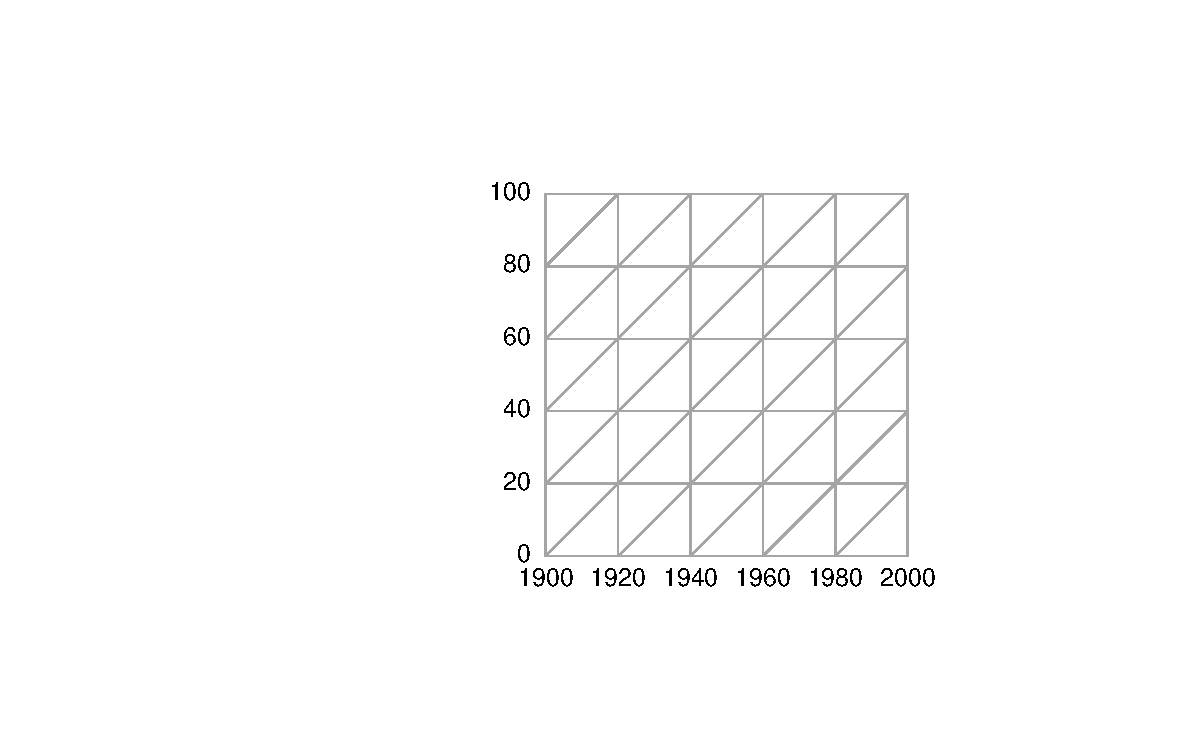
\includegraphics[scale=.7]{Figures/LabPres/APC1.pdf}
    \caption{An APC diagram}
\end{figure} 
\end{frame}

\begin{frame}
\frametitle{An old friend}
\begin{figure}[b]
    \centering
    % figure made in R/LexisStandard.R
    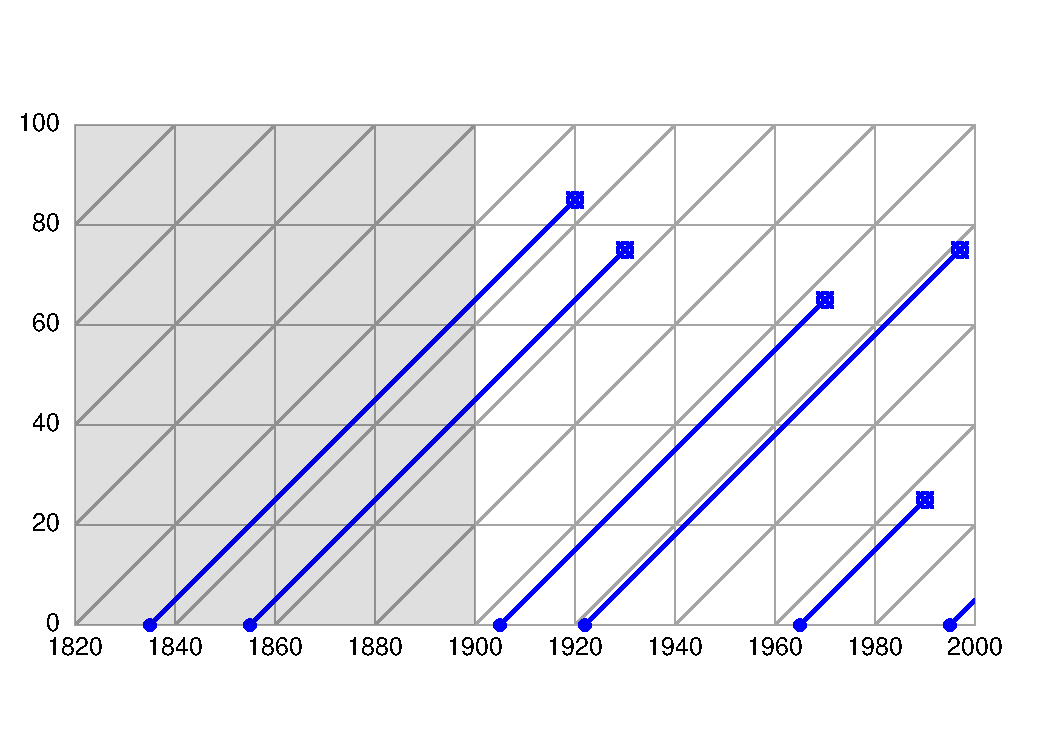
\includegraphics[scale=.7]{Figures/LabPres/APC2.pdf}
    \caption{Lifelines in the APC diagram}
\end{figure} 
\end{frame}

\section{TPD}
\begin{frame}
\frametitle{The inverse relationship}
\begin{figure}[b]
    \centering
    % figure made in R/LexisStandard.R
    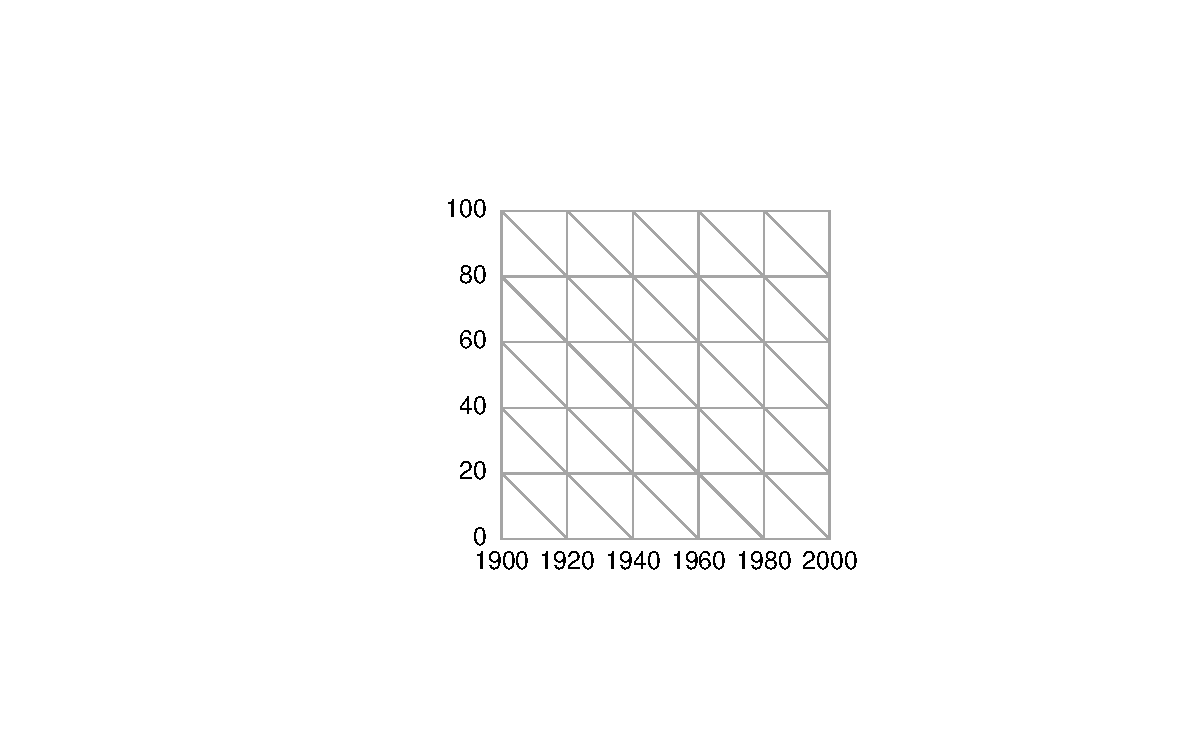
\includegraphics[scale=.7]{Figures/LabPres/TPD1.pdf}
    \caption{A TPD diagram}
\end{figure} 
\end{frame}

\begin{frame}
\frametitle{The inverse relationship}
\begin{figure}[b]
    \centering
    % figure made in R/LexisStandard.R
    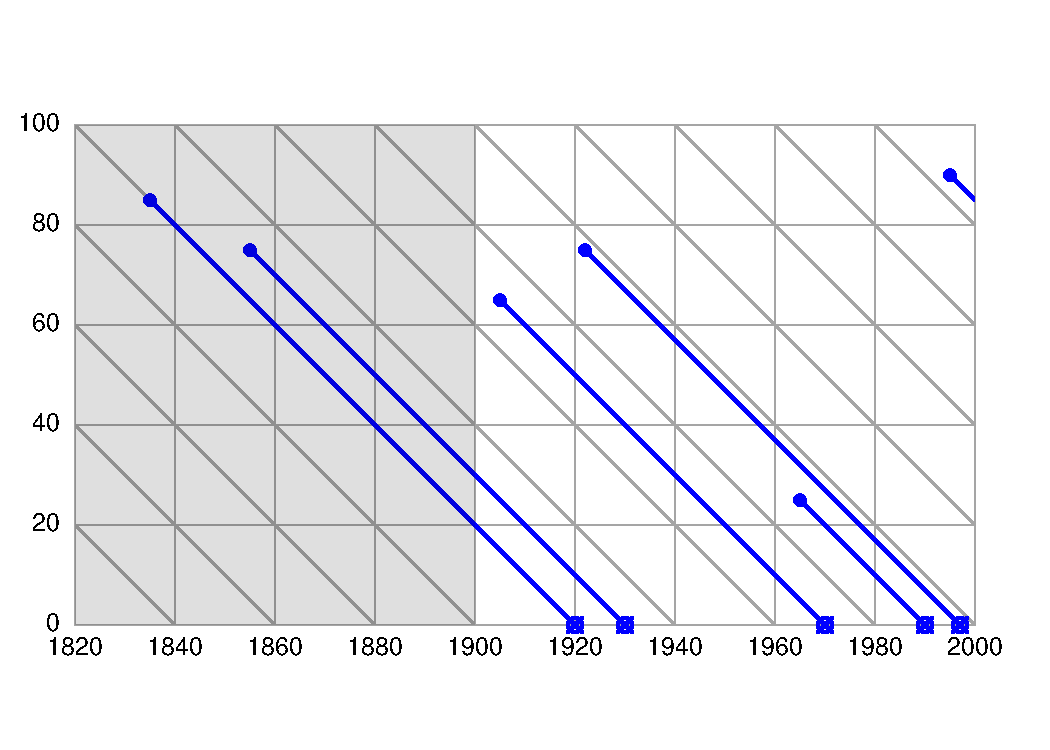
\includegraphics[scale=.7]{Figures/LabPres/TPD2.pdf}
    \caption{Lifelines in the TPD diagram}
\end{figure} 
\end{frame}

\section{TPD}

\end{document}







